\documentclass[12pt]{report}
\usepackage[utf8]{inputenc}
\usepackage{datetime}
\usepackage{amsmath}
\usepackage{ amssymb }
\usepackage{graphicx}
\usepackage[urlcolor=blue, bookmarksopen]{hyperref}
\usepackage[]{geometry}
\usepackage[]{cleveref}
\usepackage{fancyhdr}
\usepackage{xcolor}
\usepackage{siunitx}
\usepackage{ wasysym }
\usepackage{float}
\makeindex
\hypersetup{
	colorlinks=true,
	linkcolor=blue,
	filecolor=magenta,      
	urlcolor=cyan,
	citecolor=blue,
	pdftitle={Overleaf Example},
	pdfpagemode=FullScreen,
}

\urlstyle{same}
\newdate{date}{18}{10}{2025}
\title{Computer Arithmetic}
\date{\displaydate{date}}
\author{Nima Poshtiban}


\begin{document}
	\maketitle
	\tableofcontents
	\chapter{Preliminary}
\section{Radix and Base Conversion}
\paragraph{}
Digits are represented based on their \textbf{Radix}.\\
The most commonly use Radixes are \(2,\,8,\,10,\,16\), that are called Binary, Octal, Decimal and, Hexadecimal respectively.\\
A number (N) with raidx (r) can be written as\large{\[
(N)_{r} = d_{n-1} d_{n-2}\cdots\,\,d_{1}\,d_{0} . d_{-1} d_{-2} \cdots d_{-m}
\]}
where \(d_{n-1}\) is the MSB and \(d_{-m}\) is the LSB. The negative indexes are the fractional part.\\
The General Radix Conversion rule from Radix 10 to Radix (R) can be described as \[
\left(d_{n-1}\dots d_{1}d_{0}=\sum _{i=0}^{n-1}d_{i}\cdot R^{i}\right)
\]\label{conv}
It goes without saying that the conversion from R to decimal(Radix=10) is the inverted form of the formula.
\paragraph{}
There are three ways of showing a negative number. The first one is to set the \textit{MSB} if the number is negative, for example -2 with Radix of 2 can be represented as \((10000010)_{2}\) in bits. However this representation is not a proper choice because there will be twp \textit{0s}, one with positive sign and the other with negative sign.\\
\newline
Radix Complement\\
This is the most convenient way of representing a number.
The formula can be written as
\[
	N = \left(\sum_{i=0}^{digit\,length}\left(R-1\right) - i \right)\,+\,1
\]\label{rc}
where \textit{N} is the number's complement and \textit{i} is the index of the bit.\\ \\
Radix Reduced Complement\\
This one as the name suggests is similar to the \ref{rc} Equation but the final addition operation is not present in this one, this one suffers from the 0s representation, as 0 can have a set or unset sign bit.\\

\paragraph{}
In Radix \textit{r}, with the standard digit set \([0, r - 1]\), the number of digits needed to
represent the natural numbers in \([0, max]\) is \[
	\mathit{k}= \left\lfloor \log_{r}max\right\rfloor\, + 1 \,= \left\lceil log_{r}(max+1)\right\rceil
\]
With fixed-point representation using k whole and l fractional digits, We have
\[
	max = r^{k}-r^{-l}\,=r^{k} - ulp
\]
\textbf{"ulp"}stands for \textbf{unit in least significant position}, which \\For Integers \( ulp = 1 \).
\\ 
\newpage
\subsection{Problems}
\begin{enumerate}
	\item  Show the following number \label{q1} \(\left(1011 1011 1011 1010 0000  0000 0000 0000_{radix=2}\right)\) in Radix 10
	\item Write these number's with all 3 methods of Numbers\linebreak Representations: \((-38),\left(-24\right)\) and the Radix is 10.\label{q2}
	\item Calculate the result of following addition:\\
	\textbf{\textit{1F2CB00 + AFCBADO}}\label{q3}
\end{enumerate}
\subsection{Solutions}
Q\ref{q1}\, Using \eqref{conv} formula \\ 
Step 1. For simplicity convert each nibble into a hexadecimal value
\[
	\underbrace{1011}_{B}\underbrace{1011}_{B}\underbrace{1011}_{B}\underbrace{1011}_{C}\underbrace{0000}_{0}\underbrace{0000}_{0}\,=\mathsf{BBBC00h}
\]
Step 2. Now converts it into Decimal
\[
	\rightarrow 16^{5}\cdot11\,+\,16^{4}\cdot11\,+\,16^{3}\cdot11\,+\,16^{2}\cdot12\,=\,12,303,360
\]

Q\ref{q2} \begin{itemize}
	\item MSB representation: \\
	\(-38\,=\,\mathbf{0b1100110}\)\\
	\(-24\,=\,\mathbf{0b111000}\)
	\item Radix Complement \\
	\(-38\,\rightarrow\,99-38+1\,=62_{r=10}\rightarrow\,\mathbf{0b0011 1110}\)\\
	\(-24\,\rightarrow\,99-24+1\,=\,76_{r=10}\rightarrow\,\mathbf{0b0100 1100}\)\\
	\item Reduced Radix Complement\\
	\(-38\,\rightarrow\,99-38\,=61_{r=10}\rightarrow\,\mathbf{0b0011 1011}\)\\
	\(-24\,\rightarrow\,99-24\,=\,75_{r=10}\rightarrow\,\mathbf{0b0100 1011}\)\\
\end{itemize}
Q\ref{q3}
\[
\mathsf{1F2CB00 + AFCBADO\,=\,CEF85D0}
\]

\section{IEEE 754 floating point}
According to the standard a in 32bit machine a number with floating point is represented by:\textbf{ MSB is the sign bit}, \textbf{exponent}(8bit) is\[exponent +  \frac{2^{7}}{2}(bias)\] and, \textbf{23 bit for fraction} \autoref{float}
\begin{figure}[b!]
	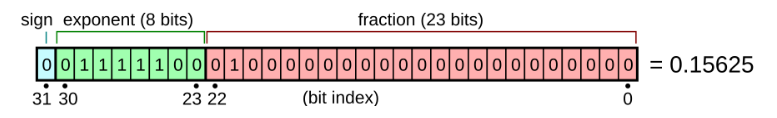
\includegraphics{float.png}
	\caption{an example of 32bit IEEE 754}
	\label{float}
\end{figure}



	\chapter{Number Representations}

\section{Dot notation}
\paragraph{} 
Extended Dot Notation
\begin{itemize}
	\item Posibit\quad  \(\newmoon\quad\in\quad \{\,\,0,\,\,\,1\}\) 
	\item Negabit\quad	\(\ocircle\quad\in\quad \{-1,0\}\)
	\item Twins
	\begin{enumerate}
		\item Unibit \quad \(\boxdot \quad\in\quad\{\,-1\,,\,1\}\)
		\item Doublebit \quad \(\blacksquare \quad\in\quad\{\,0,\,2\}\)
			\item NegaDoublebit\quad\(\square\quad \in\quad\{\,-2,0\}\)  
	\end{enumerate}

\end{itemize}

Some BSD representation using Extended Dot Notation
\begin{itemize}
	\item \textit{(n,p)} encoding \begin{align*}
		\ocircle\ocircle\ocircle\ocircle\ocircle\\
		\newmoon\,\,\newmoon\,\,\newmoon\,\newmoon\,\newmoon
	\end{align*}
	\item \textit{2's-compl, encoding}
	\begin{align*}
		\square\,\square\,\square\,\square\,\square\\
		\newmoon\,\newmoon\,\newmoon\,\newmoon\,\newmoon
	\end{align*}
	\item  \textit{2's-compl, encoding}
	\begin{align*}
		\ocircle\ocircle\ocircle\ocircle\ocircle\quad\\
		\newmoon\,\,\newmoon\,\,\newmoon\,\newmoon\,\newmoon
	\end{align*}
\end{itemize}
\paragraph{}
Unsigned positive-radix number: \begin{align*}
		\newmoon\,\newmoon\,\newmoon\,\newmoon\,\newmoon\,\newmoon\,\newmoon\,\newmoon
\end{align*}
\textit{2's Complement number}:\begin{align*}
		\ocircle\,\newmoon\,\newmoon\,\newmoon\,\newmoon\,\newmoon\,\newmoon\,\newmoon
\end{align*}
Negative-Radix number:\begin{align*}
		\ocircle\,\newmoon\,\ocircle\,\newmoon\,\ocircle\,\newmoon\,\ocircle\newmoon\,\quad
\end{align*}
Multiplication for signed numbers:
\begin{align*}
	\ocircle\quad\newmoon\quad\newmoon\quad\newmoon \\
	\mathcal{\times}\,\,\ocircle\,\,\,\,\newmoon\quad\newmoon\quad\newmoon\\
	\hline\\
	\ocircle\quad\newmoon\quad\newmoon\quad\newmoon\\
	\ocircle\quad\newmoon\quad\newmoon\quad\newmoon\quad\,\,\,\,\\
	\ocircle\quad\newmoon\quad\newmoon\quad\newmoon\qquad\quad\,\,\\
	\newmoon\quad\ocircle\quad\ocircle\quad\ocircle\quad\qquad\qquad\\
	\hline\\
	\ocircle\quad\newmoon\quad\newmoon\quad\newmoon\quad\newmoon\quad\newmoon\quad\newmoon\quad\newmoon
\end{align*}\\

Addition for unsigned positive-radix numbers:
\begin{align*}
	\ocircle\quad\newmoon\quad\newmoon\quad\newmoon \,\\
	\textbf{+}\quad\ocircle\quad\newmoon\quad\newmoon\quad\newmoon\\
	\hline
	\quad\ocircle\quad\newmoon\quad\newmoon\quad\newmoon\,\,\,\,\,\newmoon
\end{align*}\\
Multiplication for unsigned positive-radix numbers:
\begin{align*}
	\newmoon\quad\newmoon\quad\newmoon \\
	\mathcal{\times}\quad\newmoon\quad\newmoon\quad\newmoon\\
	\hline\\
	\newmoon\quad\newmoon\quad\newmoon\quad\newmoon\\
	\newmoon\quad\newmoon\quad\newmoon\quad\newmoon\quad\quad\\
	\newmoon\quad\newmoon\quad\newmoon\quad\newmoon\qquad\qquad\\
	\newmoon\quad\newmoon\quad\newmoon\quad\newmoon\qquad\qquad\qquad\\
	\hline\\
	\newmoon\quad\newmoon\quad\newmoon\quad\newmoon\quad\newmoon\quad\newmoon\quad\newmoon\quad\newmoon
\end{align*}\\
Addition for unsigned positive-radix numbers:
\begin{align*}
	\newmoon\quad\newmoon\quad\newmoon \\
	\textbf{+}\quad\newmoon\quad\newmoon\quad\newmoon\\
	\hline\\
	\quad\newmoon\quad\newmoon\quad\newmoon\quad\newmoon
\end{align*}\\
\\
There are many other number representations but the most important ones are:
\begin{enumerate}
	\item \textbf{2's} Complement
	\item \textbf{Binary Stored-carry} or \textbf{Carry-saved} format
	\item \textbf{Binary floating point number } (IEEE 754)
	\item \textbf{BCD}
\end{enumerate}

\section{Signed Number Representations}
\subsection{Signed-Magnitude Representation}
Definition: The \textbf{most left bit} is the \textbf{sign bit} (s) \[
	\mathbf{if}
\left\{\begin{array}{cl}
	s\,=\,0 & \Longrightarrow \text{positive number}\\s\,=1 & \Longrightarrow \text{negative number} 
\end{array}\right\}
\]
Numbers of this Representation type are \textit{fix-point and with no fraction}\\
In \textit{Radix r} the number \(k\)  of digits needed for representing [0,max] is
\[
	k\,=\,\left\lfloor\,log_{r}max\,+\,1 \right\rfloor\,+1\,=\,\left\lceil log_{r}(max+1) \right\rceil 
\]
\\
Example: for Radix=2 and range is [0,7] how many digits are needed?
\\\\Solution: \(k\,=\left\lceil log_{2}(7+1) \right\rceil \Longrightarrow\, 3\) so there are 3 digits are needed for representing this digit set\\\\
\textbf{Disadvantages of Signed-Magnitude Representation}
\begin{enumerate}
	\item Because of Symmetric nature of this representation there will be two \(0\)s with different signs \(\pm0\). This is unavoidable in Radix-2 Symmetric Systems.
	\item More overhead and thus more delay because of \(\pm0\) existence.
\end{enumerate}
Finally the Digit set of \textbf{Signed-Magnitude Representation} is 
\[
	\big[-(2^{k-1}\,-\,1)\,,2^{k\,-\,1}\,-1\big]
\]
\begin{figure*}
	\centering
	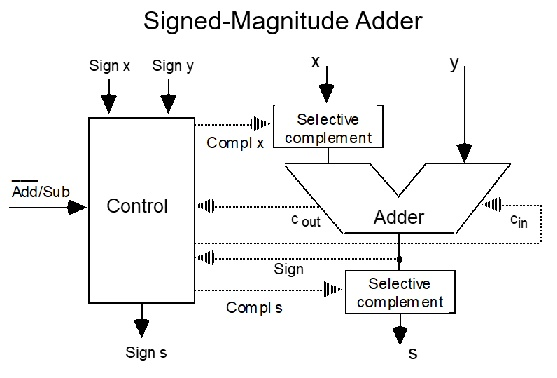
\includegraphics{smadder.jpg}
	\caption[short]{Adding signed-magnitude numbers using precomplementation and postcomplementation.}
\end{figure*}

\subsection{Biased Representations}
\paragraph{}
As the name suggests\textit{\textbf{ a bias}} is applied to the \textbf{signed number}; which then can be used for conversion from\textbf{ Signed} to \textbf{Unsigned} numbers.\\
The\textbf{ Digit set }can be shown as \( \mathbf{{[-bias,max-bias}]} \); using values from \textbf{0} to \textbf{max}, this is often called \textbf{"excess-bias"}. Most notable examples are \textbf{"excess-3" or (BCD)} and \textbf{"excess-128"} (is used for simpler hardware) coding.
Formula Demonstration:\begin{align*}
	x+y-bias=(x+bias)+(y+bias)-bias \\
	x-y+bias=(x+bias)-(y+bias)+bias\\
	\text{with kbit numbers and  a bias of } \mathbf{2^{k-1}}
\end{align*}
The Complexity is\textbf{ negligible} for this type.\\
Multiplications and Divisions become \textit{more difficult} if applied on \textbf{biased numbers}, thus the \textit{bias representation} is mostly suited for the \textbf{exponent (e)} part of \textbf{the floating-point numbers}, since they are \underline{\textbf{never}} multiplied or divided. A common example of this is \textbf{IEEE 754 standard}.
	%TODO  DIRECT AND INDIRECT SIGNED ARITHMETIC
	%TODO questions
\end{document}